\documentclass[11pt,a4paper]{article}

% ---------------------------------------------------------------
%  Authorship switch.
%  \arxivfalse : credit line as requested (you + Claude Opus 5.5).
%  \arxivtrue  : arXiv-compliant version. arXiv does not allow AI
%                tools to be listed as authors; the model is then
%                credited in a title footnote and the statement at
%                the end instead.
% ---------------------------------------------------------------
\newif\ifarxiv
\arxivfalse

\usepackage[utf8]{inputenc}
\usepackage[T1]{fontenc}
\usepackage[sc]{mathpazo}
\linespread{1.06}
\usepackage[margin=1in]{geometry}
\usepackage{microtype}
\usepackage{amsmath,amssymb,amsthm}
\usepackage{mathtools}
\usepackage{booktabs}
\usepackage{enumitem}
\usepackage[font=small,labelfont=bf]{caption}
\usepackage{xcolor}
\usepackage{tikz}
\usetikzlibrary{arrows.meta,calc}
\usepackage{pgfplots}
\pgfplotsset{compat=1.18}
\usepackage{algorithm}
\usepackage[noend]{algpseudocode}
\usepackage[most]{tcolorbox}
\usepackage{xurl}
\usepackage{needspace}
\usepackage[colorlinks=true,linkcolor=blue!50!black,citecolor=blue!50!black,urlcolor=blue!50!black]{hyperref}
\usepackage[capitalise,noabbrev]{cleveref}

\definecolor{qblue}{RGB}{37,99,235}
\definecolor{cgray}{RGB}{115,115,115}
\definecolor{direct}{RGB}{220,38,38}

\theoremstyle{plain}
\newtheorem{theorem}{Theorem}
\newtheorem{lemma}[theorem]{Lemma}
\newtheorem{corollary}[theorem]{Corollary}
\newtheorem{fact}{Fact}
\renewcommand{\thefact}{\Alph{fact}}
\theoremstyle{remark}
\newtheorem{remark}[theorem]{Remark}

\newtcolorbox{mainresult}{colback=qblue!4,colframe=qblue!60,boxrule=0.6pt,arc=2pt,left=6pt,right=6pt,top=4pt,bottom=4pt}

\newcommand{\Ostar}{O^{*}}
\newcommand{\hc}{\mathrm{hc}}
\newcommand{\GF}{\mathrm{GF}}

\title{Amplifying Determinant Sums:\\[2pt]
A Quantum Algorithm for Undirected Hamiltonicity in $\Ostar\big((8/3)^{n/2}\big)$ Time}

\ifarxiv
\author{Konstantinos Dalkafoukis\thanks{[Affiliation / e-mail.] This paper was developed with Claude Opus~5.5 (Anthropic) under the author's direction; see the contribution and AI-use statement at the end.}}
\else
\author{
  Konstantinos Dalkafoukis\thanks{Research direction, problem choice and review. Drove the project.}
  \and
  Claude Opus 5.5 (Anthropic)\thanks{AI model. Derivations, proofs, numerical checks and writing, under the direction of the first author.}
}
\fi
\date{Draft of 14 November 2026, revised 21 November 2026 --- not peer reviewed}

\begin{document}
\maketitle

\begin{abstract}
\noindent
We give a quantum algorithm that decides whether an undirected graph on $n$ vertices has a Hamiltonian cycle in time $\Ostar\big((8/3)^{n/2}\big) \subset O(1.6330^n)$. It uses $\mathrm{poly}(n)$ qubits and no quantum RAM, and its error is one-sided: it never reports a cycle that does not exist. This is below Björklund's classical bound $\Ostar(1.657^n)$, which is the fastest known algorithm for the problem, and below the $\Ostar(1.728^n)$ quantum bound of Ambainis et al.\ for the travelling salesman problem.

The algorithm runs amplitude amplification over the random choices of Björklund's determinant-sum algorithm. Cheaper repetitions shift the best trade-off between the cost of one trial and its chance of success: the cutoff on ``direct'' arcs moves from about $0.207n$ to exactly $n/6$, which gives the closed form $(8/3)^{n/2}$. The same argument applied to the narrow sieve of Björklund, Husfeldt, Kaski and Koivisto gives $\Ostar(1.6330^k)$ for the $k$-path problem.
\end{abstract}

% ===============================================================
\section{Introduction}
% ===============================================================

A Hamiltonian cycle visits every vertex of a graph exactly once. Deciding whether one exists is NP-complete, so we do not expect polynomial-time algorithms, classical or quantum. The question is how small the base $c$ of a $c^n$ running time can be.

For fifty years the best bound was the $\Ostar(2^n)$ dynamic program of Bellman and of Held and Karp~\cite{bellman,heldkarp}. Björklund broke it for undirected graphs with a Monte Carlo algorithm that runs in $\Ostar(1.657^n)$ time and polynomial space~\cite{bjorklund}.

Quantum algorithms have improved other bounds. Ambainis et al.\ combined Grover search with dynamic programming to solve the travelling salesman problem in $\Ostar(1.728^n)$, using exponentially large quantum RAM~\cite{ambainis}. Moylett, Linden and Montanaro applied quantum backtracking~\cite{montanaro} to branching algorithms for bounded-degree graphs~\cite{mlm}. None of these beats $1.657^n$ on general graphs. \Cref{tab:results} and \cref{fig:landscape} summarise the picture.

\begin{table}[t]
\centering
\small
\begin{tabular}{@{}llll@{}}
\toprule
Algorithm & Model & Graphs & Time \\
\midrule
Bellman; Held--Karp~\cite{bellman,heldkarp} & classical & general & $\Ostar(2^n)$ \\
Björklund~\cite{bjorklund} & classical, Monte Carlo & undirected & $\Ostar(1.657^n)$ \\
Björklund~\cite{bjorklund} & classical, Monte Carlo & bipartite & $\Ostar(1.415^n)$ \\
Ambainis et al.~\cite{ambainis} & quantum, exp.\ QRAM & general (TSP) & $\Ostar(1.728^n)$ \\
Moylett--Linden--Montanaro~\cite{mlm} & quantum & max degree 3 & $\Ostar(1.110^n)$ \\
 & & max degree 4 & $\Ostar(1.301^n)$ \\
 & & max degree 5--6 & $\Ostar(1.680^n)$ \\
\textbf{This paper} & \textbf{quantum, poly qubits} & \textbf{undirected} & $\boldsymbol{\Ostar(1.6330^n)}$ \\
\bottomrule
\end{tabular}
\caption{Exponential-time algorithms for Hamiltonicity. $\Ostar$ hides polynomial factors.}
\label{tab:results}
\end{table}

\begin{mainresult}
\begin{theorem}\label{thm:main}
There is a quantum algorithm that, given an undirected graph $G$ on $n$ vertices, runs in time $\Ostar\big((8/3)^{n/2}\big) \subset O(1.6330^n)$ using $\mathrm{poly}(n)$ qubits and no QRAM.
\begin{itemize}[nosep,leftmargin=1.5em]
  \item If $G$ has no Hamiltonian cycle, it always answers ``no''.
  \item If $G$ has a Hamiltonian cycle, it answers ``yes'' with probability at least $2/3$.
\end{itemize}
The same holds for Hamiltonian path, and a cycle can be found with polynomial overhead.
\end{theorem}
\begin{corollary}\label[corollary]{cor:kpath}
The undirected $k$-path problem can be decided by a quantum algorithm with one-sided error in time $\Ostar\big((8/3)^{k/2}\big)\cdot\mathrm{poly}(n) \subset O(1.6330^k)\cdot\mathrm{poly}(n)$.
\end{corollary}
\end{mainresult}

\paragraph{The idea in one paragraph.}
Björklund's algorithm repeats a randomized test. Each test picks a random half/half partition of the vertices and evaluates an algebraic sum that costs $2^{n/2+m}$. The test detects a Hamiltonian cycle only if the cycle has at most $m$ \emph{direct} arcs, meaning arcs with both ends in the first half, and for small $m$ that happens with exponentially small probability $P$. Classically one needs about $1/P$ tests; amplitude amplification needs only $1/\sqrt{P}$. Because a rare event now costs less, the quantum algorithm can afford a smaller cutoff $m$, which makes each test cheaper. Re-optimising moves the cutoff from $0.207n$ to $n/6$ (\cref{fig:tradeoff}).

\paragraph{Relation to the Exponential Time Hypothesis.}
Our result lowers the base of the exponent. It does not give a subexponential algorithm and is fully consistent with ETH.

\paragraph{Organisation.}
\Cref{sec:prelim} recalls the parts of Björklund's framework we need. \Cref{sec:algorithm} describes the quantum algorithm and \cref{sec:analysis} proves \cref{thm:main}. \Cref{sec:extensions} covers extensions, including \cref{cor:kpath}, and \cref{sec:numerics} reports numerical checks. \Cref{sec:limits} lists limitations and open problems.

\begin{figure}[t]
\centering
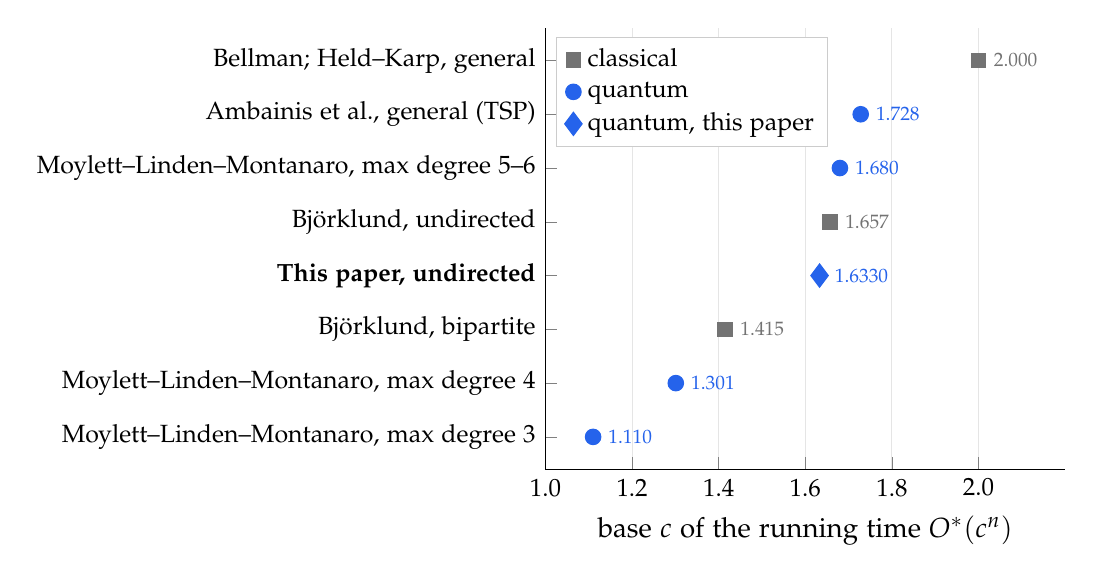
\begin{tikzpicture}
\begin{axis}[
  scale only axis, width=6.6cm, height=5.6cm,
  xmin=1.0, xmax=2.2,
  xtick={1.0,1.2,1.4,1.6,1.8,2.0},
  xticklabel style={font=\small,/pgf/number format/fixed,/pgf/number format/precision=1,/pgf/number format/fixed zerofill},
  ymin=0.4, ymax=8.6,
  ytick={1,2,3,4,5,6,7,8},
  yticklabels={
    {Moylett--Linden--Montanaro, max degree 3},
    {Moylett--Linden--Montanaro, max degree 4},
    {Björklund, bipartite},
    {\textbf{This paper, undirected}},
    {Björklund, undirected},
    {Moylett--Linden--Montanaro, max degree 5--6},
    {Ambainis et al., general (TSP)},
    {Bellman; Held--Karp, general}},
  yticklabel style={font=\small},
  xlabel={base $c$ of the running time $\Ostar(c^n)$},
  xmajorgrids, grid style={gray!20},
  axis y line*=left, axis x line*=bottom,
  legend style={at={(0.02,0.98)},anchor=north west,font=\small,draw=gray!40},
  legend cell align=left,
  every node near coord/.append style={font=\scriptsize,anchor=west,xshift=2pt},
]
\addplot[only marks, mark=square*, mark size=2.6pt, cgray,
  nodes near coords, point meta=x, nodes near coords={\pgfmathprintnumber[fixed,fixed zerofill,precision=3]{\pgfplotspointmeta}}]
  coordinates {(1.415,3) (1.657,5) (2.000,8)};
\addlegendentry{classical}
\addplot[only marks, mark=*, mark size=2.8pt, qblue,
  nodes near coords, point meta=x, nodes near coords={\pgfmathprintnumber[fixed,fixed zerofill,precision=3]{\pgfplotspointmeta}}]
  coordinates {(1.110,1) (1.301,2) (1.680,6) (1.728,7)};
\addlegendentry{quantum}
\addplot[only marks, mark=diamond*, mark size=4.2pt, qblue,
  nodes near coords, point meta=x, nodes near coords={\textbf{\pgfmathprintnumber[fixed,fixed zerofill,precision=4]{\pgfplotspointmeta}}}]
  coordinates {(1.6330,4)};
\addlegendentry{quantum, this paper}
\end{axis}
\end{tikzpicture}
\caption{Known bases for Hamiltonicity. On general undirected graphs, the previous best quantum algorithm (1.728) was slower than the best classical one (1.657). Our algorithm (1.6330) is faster than both. For maximum degree~3 or~4, quantum backtracking~\cite{mlm} remains much faster.}
\label{fig:landscape}
\end{figure}

% ===============================================================
\section{Preliminaries}\label{sec:prelim}
% ===============================================================

\paragraph{Notation.}
$\Ostar(\cdot)$ hides factors polynomial in $n$. $H(x) = -x\log_2 x - (1-x)\log_2(1-x)$ is the binary entropy. We assume $n$ is even; for odd $n$, take parts of sizes $\lceil n/2\rceil$ and $\lfloor n/2\rfloor$, which does not change the base.

\paragraph{Direct arcs.}
Fix a balanced partition $V = V_1 \cup V_2$, $|V_1| = |V_2| = n/2$. Walking around a Hamiltonian cycle, call an arc \emph{direct} if both its ends lie in $V_1$ (\cref{fig:partition}). Let $\hc^m(G)$ be the set of Hamiltonian cycles with exactly $m$ direct arcs.

\begin{figure}[t]
\centering
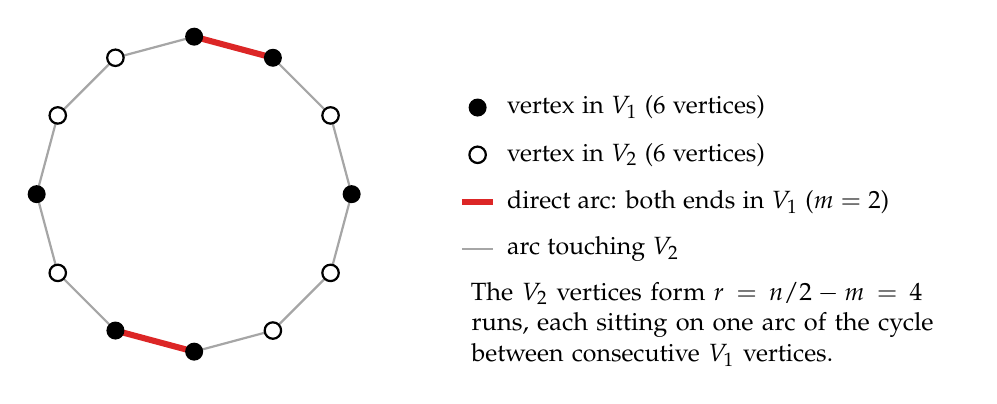
\begin{tikzpicture}[scale=1.0,
  v1/.style={circle,fill=black,inner sep=2.3pt},
  v2/.style={circle,draw=black,fill=white,inner sep=2.1pt,thick}]
  \def\R{2.0}
  % pattern around the cycle: 1 = V1, 0 = V2
  \foreach \i/\t in {0/1,1/1,2/0,3/1,4/0,5/0,6/1,7/1,8/0,9/1,10/0,11/0} {
    \coordinate (p\i) at ({90-30*\i}:\R);
  }
  % ordinary arcs
  \foreach \i/\j in {1/2,2/3,3/4,4/5,5/6,7/8,8/9,9/10,10/11,11/0} {
    \draw[gray!70, thick] (p\i) -- (p\j);
  }
  % direct arcs
  \draw[direct, line width=2.2pt] (p0) -- (p1);
  \draw[direct, line width=2.2pt] (p6) -- (p7);
  \foreach \i in {0,1,3,6,7,9} { \node[v1] at (p\i) {}; }
  \foreach \i in {2,4,5,8,10,11} { \node[v2] at (p\i) {}; }
  % legend
  \begin{scope}[xshift=3.6cm, yshift=1.1cm]
    \node[v1] at (0,0) {}; \node[anchor=west,font=\small] at (0.25,0) {vertex in $V_1$ (6 vertices)};
    \node[v2] at (0,-0.6) {}; \node[anchor=west,font=\small] at (0.25,-0.6) {vertex in $V_2$ (6 vertices)};
    \draw[direct, line width=2.2pt] (-0.2,-1.2) -- (0.2,-1.2); \node[anchor=west,font=\small] at (0.25,-1.2) {direct arc: both ends in $V_1$ ($m = 2$)};
    \draw[gray!70, thick] (-0.2,-1.8) -- (0.2,-1.8); \node[anchor=west,font=\small] at (0.25,-1.8) {arc touching $V_2$};
    \node[anchor=west,font=\small,align=left,text width=6.2cm] at (-0.2,-2.75) {The $V_2$ vertices form $r = n/2 - m = 4$ runs, each sitting on one arc of the cycle between consecutive $V_1$ vertices.};
  \end{scope}
\end{tikzpicture}
\caption{A Hamiltonian cycle on $n = 12$ vertices under a balanced partition. Björklund's test with cutoff $m_{\max}$ detects this cycle only if it has at most $m_{\max}$ direct arcs. A smaller cutoff makes each test cheaper but the event rarer.}
\label{fig:partition}
\end{figure}

\subsection{Björklund's determinant sums}

Björklund builds a bidirected graph $D$ on $V_1$ and a label set $L = V_2 \cup L_m$, where $L_m$ holds $m$ extra labels, so $|L| = n/2 + m$~\cite[\S 3.2]{bjorklund}. Each edge of $G$ gets a formal variable over a field $\GF(2^k)$ of characteristic two. The \emph{labelled cycle cover sum} is
\[
  \Lambda(D, L, f) \;=\; \sum_{C \in \mathrm{cc}(D)} \;\sum_{g\colon L \twoheadrightarrow C} \;\prod_{a \in C} f\big(a, g^{-1}(a)\big),
\]
where $\mathrm{cc}(D)$ is the set of cycle covers of $D$ and $g$ ranges over surjections. For an arc $uv$ and $X \subseteq V_2$, $f(uv, X)$ sums the variable products of $u$--$v$ paths in $G$ that pass through exactly the vertices of $X$. For an edge $uv$ inside $V_1$ and $d \in L_m$, $f(uv,\{d\}) = x_{uv,d}$. We use four facts.

\begin{fact}[{\cite[Lemma 9]{bjorklund}}]\label{fact:zero}
$\Lambda(D, V_2 \cup L_m, f)$ is the zero polynomial if and only if $\hc^m(G) = \emptyset$.
\end{fact}

\begin{fact}[{\cite[Lemma 10]{bjorklund}}]\label{fact:prob}
If $G$ is Hamiltonian and the balanced partition is uniformly random, then
\[
  \Pr\big[\hc^m(G) \neq \emptyset\big] \;\ge\; \binom{n/2-1}{m-1}^{\!2} \Big/ \binom{n}{n/2}.
\]
\end{fact}
\noindent
\Cref{app:count} gives the exact probability that a fixed cycle has $m$ direct arcs; it has the same exponential rate.

\begin{fact}[{\cite[\S 4 and Lemma 11]{bjorklund}}]\label{fact:space}
Replacing paths by walks gives a function $g(\cdot,\cdot,r)$ and the polynomial
\[
  q(g, r) \;=\; \sum_{Y \subseteq L} \det\Big(\sum_{Z \subseteq Y} \mathbf{M}_{g(\cdot,\cdot,r)}(Z)\Big),
  \qquad
  [r^{|L|}]\, q(g,r) \;=\; [r^{|L|}]\, p(f,r) \;=\; \Lambda .
\]
For fixed $Y$ and $r$, the inner $(n/2)\times(n/2)$ matrix is computed in polynomial time and space by counting weighted walks. Evaluating $q$ at $|L|\cdot n$ values of $r$ and interpolating recovers $\Lambda$, provided the field has more than $|L|\cdot n$ elements.
\end{fact}
\noindent
So, with the variables set to field elements, one evaluation of $\Lambda$ costs $\Ostar(2^{|L|}) = \Ostar(2^{n/2+m})$ time and only polynomial space. Björklund's $1.657^n$ analysis uses an exponential-space table, but its dominant $2^{|L|}$ factor is the same.

\begin{fact}[Schwartz--Zippel]\label{fact:sz}
$\Lambda$ has degree at most $n$ in the edge variables. At a uniformly random point of $\GF(2^k)^N$ with $2^k \ge 4n$, a nonzero $\Lambda$ evaluates to a nonzero value with probability at least $3/4$.
\end{fact}

\paragraph{The classical algorithm.}
Björklund repeats the test for every $m \le m_{\max}$ over many random partitions. He takes $m_{\max} \approx 0.205n$ and about $2^{0.024n}$ repetitions, which gives $\Ostar(1.657^n)$~\cite[\S 3.2.2]{bjorklund}.

\subsection{Quantum tools}

\begin{lemma}[Amplitude amplification~\cite{bhmt}]\label[lemma]{lem:aa}
Let $A$ be a unitary with
\[
  A|0\rangle = \sqrt{a}\,|\mathrm{good}\rangle + \sqrt{1-a}\,|\mathrm{bad}\rangle,
\]
where a flag qubit marks the good part. If $a \ge a_0$ for a known $a_0 > 0$, then $O(1/\sqrt{a_0})$ applications of $A$, $A^\dagger$ and two reflections produce a good outcome with probability at least $2/3$. Since $a$ itself is unknown, this uses the randomised iteration counts of~\cite[Theorem~3]{bhmt}, stopped after $O(1/\sqrt{a_0})$ applications. If $a = 0$, no outcome is ever good.
\end{lemma}

\paragraph{Reversible computation.}
A classical computation running in polynomial time can be made reversible with polynomially many gates and ancillas: compute, copy the result, uncompute. Addition in a field of characteristic two is bitwise XOR, so adding a value into an accumulator is itself reversible.

% ===============================================================
\section{The algorithm}\label{sec:algorithm}
% ===============================================================

One coherent run $A$ evaluates Björklund's test on a superposition of all its random choices (\cref{alg:run}). Amplitude amplification then repeats $A$ about $2^{0.041n}$ times (\cref{alg:main}).

\paragraph{Parameters.}
$m_{\max} = \lceil n/6 \rceil$ (optimised in \cref{sec:analysis}) and $k = 2\lceil \log_2 n\rceil + 2$, so that $2^k \ge 4n^2$. This is large enough both for interpolation at $|L|\cdot n$ points (\cref{fact:space}) and for \cref{fact:sz}.

\paragraph{Registers.}
\begin{itemize}[nosep]
  \item $P$: $n$ qubits; bit $i$ is $1$ if vertex $i$ is in $V_1$.
  \item $X$: one $k$-qubit field element for every variable any partition might use: $x_{uv}$ for each ordered pair and $x_{uv,d}$ for each ordered pair and each $d \le m_{\max}$. That is at most $n^3$ variables, so $O(n^3 \log n)$ qubits.
  \item Workspace of polynomial size, a balance bit $b$, test bits $t_0,\dots,t_{m_{\max}}$ and the flag $F$.
\end{itemize}

\begin{algorithm}[t]
\caption{One coherent run $A$ (sets the flag $F$)}\label{alg:run}
\begin{algorithmic}[1]
\State Apply $H^{\otimes n}$ to $P$; compute $b \gets [\,P \text{ has exactly } n/2 \text{ ones}\,]$
\State Apply Hadamards to $X$ \Comment{uniform superposition of evaluation points}
\For{$m = 0, 1, \dots, m_{\max}$}
  \State $L \gets V_2(P) \cup L_m$ \Comment{$|L| = n/2 + m$ on branches with $b = 1$}
  \For{$j = 1, \dots, |L|\cdot n$} \Comment{interpolation points $r_j$}
    \State $\mathit{acc}_j \gets 0$
    \For{all $Y \subseteq L$} \Comment{$|L|$-bit counter}
      \State compute $N \gets \sum_{Z\subseteq Y}\mathbf{M}_{g}(Z)$ at $(X, r_j)$ \Comment{walk counts, poly time}
      \State $\mathit{acc}_j \gets \mathit{acc}_j \oplus \det(N)$; uncompute $N$ \Comment{XOR in $\GF(2^k)$}
    \EndFor
  \EndFor
  \State $\Lambda_m \gets \sum_j c_j\, \mathit{acc}_j$ \Comment{fixed Lagrange coefficients}
  \State $t_m \gets [\,\Lambda_m \neq 0\,]$
\EndFor
\State $F \gets b \wedge (t_0 \vee \dots \vee t_{m_{\max}})$
\end{algorithmic}
\end{algorithm}

\begin{algorithm}[t]
\caption{Quantum Hamiltonicity test}\label{alg:main}
\begin{algorithmic}[1]
\State $a_0 \gets \Pr[b=1]\cdot \tfrac34 \cdot \binom{n/2-1}{m_{\max}-1}^{2} \big/ \binom{n}{n/2}$ \Comment{lower bound of \cref{lem:complete}}
\State Run amplitude amplification on $A$ with randomised iteration counts (\cref{lem:aa}), using at most $O(1/\sqrt{a_0})$ applications of $A$, and measure $F$ after each round
\State \Return ``yes'' if some measured $F = 1$, otherwise ``no''
\end{algorithmic}
\end{algorithm}

\paragraph{Cost of one run.}
Each step inside the loops is a polynomial-time classical computation made reversible, and the counter increment $x \mapsto x+1$ is a permutation. So
\[
  \mathrm{gates}(A) \;=\; \sum_{m=0}^{m_{\max}} |L|\, n\cdot 2^{\,n/2+m}\cdot \mathrm{poly}(n) \;=\; \Ostar\big(2^{\,n/2+m_{\max}}\big),
\]
and $A$ uses $\mathrm{poly}(n)$ qubits. On branches with $b = 0$ the computation is irrelevant, because $F = 0$ there.

\begin{remark}
The circuit depth is exponential, as for any exponential-time algorithm. The workspace stays entangled with the flag after a run. This is harmless: amplitude amplification reflects only on $F$ and applies $A$ and $A^\dagger$ as black boxes. A Dicke-state preparation~\cite{dicke} would remove the $\Theta(1/\sqrt n)$ factor $\Pr[b=1]$, but this changes only polynomial factors.
\end{remark}

% ===============================================================
\section{Analysis}\label{sec:analysis}
% ===============================================================

Let $a$ be the probability that measuring $F$ after $A|0\rangle$ gives $1$.

\begin{lemma}[Soundness]\label[lemma]{lem:sound}
If $G$ has no Hamiltonian cycle, then $a = 0$.
\end{lemma}
\begin{proof}
Every set $\hc^m(G)$ is empty, for every partition. By \cref{fact:zero} every $\Lambda_m$ is the zero polynomial, so $\Lambda_m(P,X) = 0$ for all values of $P$ and $X$. Hence every $t_m = 0$, and $F = 0$ on every branch.
\end{proof}

\begin{lemma}[Completeness]\label[lemma]{lem:complete}
If $G$ has a Hamiltonian cycle, then with $m^\ast = m_{\max}$,
\[
  a \;\ge\; a_0 \;:=\; \Pr[b=1]\cdot\frac34\cdot\binom{n/2-1}{m^\ast-1}^{\!2}\Big/\binom{n}{n/2},
  \qquad \Pr[b=1] = \Theta(n^{-1/2}).
\]
\end{lemma}
\begin{proof}
Measuring $P$ and $X$ after $A$ gives an independent uniform bit string and a uniform evaluation point. Given $b=1$, $P$ is a uniform balanced partition. By \cref{fact:prob}, $\hc^{m^\ast}(G)\ne\emptyset$ with at least the stated probability, and then $\Lambda_{m^\ast}$ is a nonzero polynomial by \cref{fact:zero}. $X$ is independent of $P$, so by \cref{fact:sz}, $\Lambda_{m^\ast}(P,X)\ne 0$ with probability at least $3/4$. In that event $t_{m^\ast}=1$ and $F=1$.
\end{proof}

\begin{proof}[Proof of \cref{thm:main}]
Run \cref{alg:main}. By \cref{lem:sound} it never answers ``yes'' wrongly. By \cref{lem:complete} and \cref{lem:aa}, a Hamiltonian $G$ gives ``yes'' with probability at least $2/3$. The total cost is
\[
  T(n) \;=\; O\!\left(\frac{1}{\sqrt{a_0}}\right)\cdot \Ostar\!\left(2^{\,n/2+m_{\max}}\right),
\]
which \cref{lem:opt} below evaluates. For Hamiltonian path, add a vertex adjacent to every vertex: the new graph on $n+1$ vertices has a Hamiltonian cycle if and only if $G$ has a Hamiltonian path. Finding a cycle is treated in \cref{sec:extensions}.
\end{proof}

\begin{lemma}[Optimisation]\label[lemma]{lem:opt}
With $m_{\max} = \mu n$, $\frac1n \log_2 T(n) \to \varphi(\mu)$, where
\[
  \varphi(\mu) \;=\; \tfrac12 + \mu + \tfrac12\big(1 - H(2\mu)\big).
\]
$\varphi$ is minimised at $\mu = 1/6$, where $2^{\varphi(1/6)} = \sqrt{8/3} \approx 1.63299$.
\end{lemma}
\begin{proof}
By Stirling's formula, $\log_2\binom{n/2}{\mu n} = \tfrac n2 H(2\mu) + O(\log n)$ and $\log_2\binom{n}{n/2} = n - O(\log n)$, so $\log_2(1/a_0) = n\big(1 - H(2\mu)\big) + O(\log n)$. Since $H$ is concave, $\varphi$ is convex. Its derivative is
\[
  \varphi'(\mu) \;=\; 1 - H'(2\mu) \;=\; 1 - \log_2\frac{1-2\mu}{2\mu},
\]
which vanishes when $(1-2\mu)/(2\mu) = 2$, that is $\mu = 1/6$. Using $H(1/3) = \log_2 3 - \tfrac23$,
\[
  \varphi(1/6) \;=\; \tfrac23 + \tfrac12\Big(\tfrac53 - \log_2 3\Big) \;=\; \tfrac32 - \tfrac12\log_2 3,
  \qquad
  2^{\varphi(1/6)} \;=\; \frac{2^{3/2}}{\sqrt3} \;=\; \sqrt{8/3}. \qedhere
\]
\end{proof}

\begin{figure}[t]
\centering
\begin{tikzpicture}
\begin{axis}[
  width=0.9\linewidth, height=6.6cm,
  xmin=0.05, xmax=0.35, ymin=1.60, ymax=1.80,
  xtick={0.05,0.10,0.15,0.20,0.25,0.30,0.35},
  xticklabel style={/pgf/number format/fixed,/pgf/number format/precision=2,/pgf/number format/fixed zerofill},
  yticklabel style={/pgf/number format/fixed,/pgf/number format/precision=2,/pgf/number format/fixed zerofill},
  xlabel={cutoff on direct arcs, $\mu = m_{\max}/n$},
  ylabel={base $c$ of the total cost $c^{n}$},
  ylabel style={font=\small}, xlabel style={font=\small},
  ticklabel style={font=\small},
  grid=major, grid style={gray!18},
  legend style={at={(0.52,0.97)},anchor=north,font=\small,draw=gray!40},
  legend cell align=left,
  clip=true,
]
\addplot[cgray, very thick] table[x=mu,y=classical]{figs/curves.dat};
\addlegendentry{classical: cost $2^{n/2+m}/P$}
\addplot[qblue, very thick] table[x=mu,y=quantum]{figs/curves.dat};
\addlegendentry{quantum: cost $2^{n/2+m}/\sqrt{P}$}
\draw[cgray, dashed] (axis cs:0.207107,1.60) -- (axis cs:0.207107,1.656854);
\draw[qblue, dashed] (axis cs:0.166667,1.60) -- (axis cs:0.166667,1.632993);
\addplot[only marks, mark=square*, mark size=2.6pt, cgray] coordinates {(0.207107,1.656854)};
\addplot[only marks, mark=*, mark size=2.8pt, qblue] coordinates {(0.166667,1.632993)};
\node[anchor=west,font=\footnotesize,align=left,text=cgray!80!black] (cl) at (axis cs:0.255,1.652) {Björklund's optimum\\$\mu\approx 0.207$, base $1.6569$};
\node[anchor=west,font=\footnotesize,align=left,text=qblue!80!black] (qu) at (axis cs:0.255,1.618) {our optimum\\$\mu = 1/6$, base $1.6330$};
\draw[-{Stealth[length=5pt]}, cgray] (cl.west) -- (axis cs:0.2105,1.6572);
\draw[-{Stealth[length=5pt]}, qblue] (qu.west) -- (axis cs:0.1700,1.6326);
\end{axis}
\end{tikzpicture}
\caption{The trade-off behind \cref{thm:main}. A larger cutoff makes each test more likely to succeed but more expensive. Amplitude amplification halves the cost of rare successes, so the optimum moves to the left, from $\mu \approx 0.207$ to $\mu = 1/6$, and the base drops from $1.6569$ to $1.6330$.}
\label{fig:tradeoff}
\end{figure}

\paragraph{Why the optimum moves.}
Classically the repetitions cost $1/a_0$ instead of $1/\sqrt{a_0}$, which gives the exponent $\psi(\mu) = \tfrac12 + \mu + 1 - H(2\mu)$. Its stationarity condition is $H'(2\mu) = 1/2$ rather than $1$, so $2\mu = \sqrt2 - 1$, $\mu \approx 0.2071$ and $2^{\psi} \approx 1.6569$, recovering Björklund's bound. In both cases one more unit of cutoff doubles the cost of a test. Classically that is balanced against the full gain in success probability; quantumly only the square root of the gain counts, so the balance point is reached sooner (\cref{fig:tradeoff}).

\paragraph{Unbalanced partitions do not help.}
Björklund's reduction works for any partition, with cost $2^{|V_2|+m}$. With $|V_1| = \alpha n$, counting cyclic arrangements (as in \cref{app:count}) gives the success exponent $\alpha H(\mu/\alpha) + (1-\alpha) H\big((\alpha-\mu)/(1-\alpha)\big) - H(\alpha)$. Numerical optimisation over $(\alpha,\mu)$ returns $\alpha = 1/2$, both classically and quantumly.

% ===============================================================
\section{Extensions}\label{sec:extensions}
% ===============================================================

The amplification applies wherever an algebraic sieve repeats a one-sided random trial.

\paragraph{Finding a cycle.}
A ``yes'' answer is always correct, so self-reduction is safe. For each edge $e$ in turn, test $G - e$ with $O(\log n)$ repetitions and delete $e$ if any test says ``yes''. A wrong ``no'' only keeps an edge we could have deleted, and the repetitions make this unlikely for all edges at once. At the end every remaining edge is needed, so the remaining graph is a Hamiltonian cycle. The overhead is polynomial.

\paragraph{The $k$-path problem (\cref{cor:kpath}).}
The narrow sieve of Björklund, Husfeldt, Kaski and Koivisto~\cite{bhkk} has the same structure. It picks a uniformly random ordered partition $(V_1,V_2)$ of all $n$ vertices. One trial sums over $2^{k_1+\ell_2}$ terms in polynomial space, with $k_1 = \gamma_1 k$ and $\ell_2 = \gamma_2 k$, and it never reports a false positive. A fixed $k$-path is admissible with probability~\cite[Lemma 7]{bhkk}
\[
  P(k,k_1,\ell_2) \;=\; 2^{-k}\binom{k_1+1}{k-k_1-\ell_2}\binom{k-k_1-1}{\ell_2}.
\]
Classically they take $\gamma_1 = 0.5$ and $\gamma_2 = 0.207107$, giving $1.6569^k$. With amplitude amplification, the cost $2^{k_1+\ell_2}/\sqrt{P}$ is minimised at $\gamma_1 = 1/2$ and $\gamma_2 = 1/6$. At $\gamma_1 = 1/2$ the formula has the same exponential rate as \cref{fact:prob}, so the base is again $\sqrt{8/3}$. Our classical model reproduces their parameters to six digits.

\paragraph{Bounded-degree graphs.}
For maximum degree 5 or 6, \cref{thm:main} improves the quantum bound from $\Ostar(1.680^n)$~\cite{mlm} to $\Ostar(1.6330^n)$. For maximum degree 3 or 4, the bounds $\Ostar(1.110^n)$ and $\Ostar(1.301^n)$ of~\cite{mlm} remain better.

\paragraph{Where amplification does not help.}
Björklund's $\Ostar(2^{n/2})$ algorithm for bipartite graphs, and his $\Ostar(2^{n-i})$ variant given an independent set of size $i$, use a fixed partition. There is no random trial to amplify.

\paragraph{Weighted TSP.}
Björklund handles positive integer edge weights with one extra indeterminate $y$ that records the total weight~\cite[\S 5]{bjorklund}. The coefficient of $y^l$ is nonzero only if a Hamiltonian cycle of weight $l$ exists, and a fast Fourier transform over $\GF(2^k)$ with $2^k > w$ recovers all coefficients, where $w$ is the sum of all weights. A run then costs $\Ostar(w\cdot 2^{n/2+m})$ and stays one-sided for the question ``is there a tour of weight at most $W$?'' Amplifying it as in \cref{alg:main} gives $\Ostar\big(w\,(8/3)^{n/2}\big)$ for that question, and binary search over $W$ finds the optimum with $O(\log w)$ more runs. This compares with Björklund's classical $\Ostar(w\cdot 1.657^n)$.

% ===============================================================
\section{Numerical checks}\label{sec:numerics}
% ===============================================================

\Cref{fig:convergence} evaluates the exponent with exact binomial coefficients instead of Stirling's formula. The optimal finite-$n$ base decreases monotonically to $\sqrt{8/3}$ and stays below the classical curve at every $n$. Three further checks:
\begin{itemize}[nosep]
  \item \textbf{Counting formula.} For $n = 24$, $2\times 10^5$ random balanced partitions give a direct-arc distribution that matches the exact formula of \cref{app:count} to within $0.0016$ at every $m$ (\cref{fig:mc}).
  \item \textbf{$k$-path.} Exact binomials at $k = 3000$ give a quantum base of $1.6349$, converging to $\sqrt{8/3}$.
  \item \textbf{Björklund's test end to end.} \texttt{bjorklund\_check.py} implements the test over $\GF(2^{16})$ on small graphs with $n \le 10$, for every balanced partition and every $m$. It covers random graphs, two hand-made graphs (one of them non-Hamiltonian) and the cycles $C_8$ and $C_{10}$. In all $2{,}560$ cases, $\Lambda$ computed through Lemma~6 of~\cite{bjorklund} equals the closed form of \cref{fact:zero} at the same random point. On the random and hand-made graphs, the polynomial-space route through walks (\cref{fact:space}) gives the same value too. The test was never nonzero without a Hamiltonian cycle with $m$ direct arcs, and never zero with one. On $C_8$ and $C_{10}$ it fires on exactly the partitions counted by \cref{lem:count}.
\end{itemize}
Scripts are listed in \cref{app:repro}.

\begin{figure}[t]
\centering
\begin{tikzpicture}
\begin{axis}[
  width=0.78\linewidth, height=6.2cm,
  xmode=log, log basis x=10,
  xmin=50, xmax=14000, ymin=1.62, ymax=1.70,
  xtick={60,200,1000,4000,12000},
  xticklabels={60,200,1000,4000,12000},
  xlabel={number of vertices $n$ (log scale)},
  ylabel={optimal base at this $n$},
  ticklabel style={font=\small}, xlabel style={font=\small}, ylabel style={font=\small},
  yticklabel style={/pgf/number format/fixed,/pgf/number format/precision=2,/pgf/number format/fixed zerofill},
  grid=major, grid style={gray!18},
  legend style={at={(0.97,0.97)},anchor=north east,font=\small,draw=gray!40},
  legend cell align=left,
  clip=false,
]
\addplot[cgray, thick, mark=square*, mark size=1.8pt] table[x=n,y=classical]{figs/convergence.dat};
\addlegendentry{classical, exact binomials}
\addplot[qblue, thick, mark=*, mark size=1.9pt] table[x=n,y=quantum]{figs/convergence.dat};
\addlegendentry{quantum, exact binomials}
\draw[cgray, dashed] (axis cs:50,1.656854) -- (axis cs:14000,1.656854);
\draw[qblue, dashed] (axis cs:50,1.632993) -- (axis cs:14000,1.632993);
\node[anchor=west,font=\small,text=cgray!80!black] at (axis cs:14500,1.656854) {$1.6569$};
\node[anchor=west,font=\small,text=qblue!80!black] at (axis cs:14500,1.632993) {$\sqrt{8/3}$};
\end{axis}
\end{tikzpicture}
\caption{Convergence of the exact finite-$n$ optimum to the asymptotic bases (dashed). At $n = 12{,}000$ the quantum base is $1.6333$.}
\label{fig:convergence}
\end{figure}

% ===============================================================
\section{Limitations and open problems}\label{sec:limits}
% ===============================================================

The argument is short because it reuses published lemmas. Three points need checking before the result can be claimed.
\begin{enumerate}[nosep]
  \item \textbf{Novelty.} Searches in November 2026 found no quantum bound below $1.657^n$ for undirected Hamiltonicity, and none below $1.657^k$ for $k$-path. Amplifying a Monte Carlo algorithm is standard, so the observation may be folklore. Experts should be consulted before any claim of priority.
  \item \textbf{Polynomial-space running time.} Björklund states the polynomial-space variant but not its total running time. Our bound of $2^{|L|}\cdot\mathrm{poly}(n)$ per run follows from his \S 4. There, each of the $2^{|L|}$ terms is a polynomial-time walk count followed by a determinant, evaluated at $|L|\cdot n$ interpolation points. We have checked this against his text; an expert should still confirm it.
  \item \textbf{Reliance on published lemmas.} We use Lemmas 9--11 of~\cite{bjorklund} and Lemma 7 of~\cite{bhkk} as published and have not re-proved them. We tested Björklund's lemmas end to end on small graphs (\cref{sec:numerics}), but tests on small graphs are not a proof.
\end{enumerate}

\paragraph{Cost model.}
The algorithm needs $\mathrm{poly}(n)$ logical qubits (the evaluation point alone uses $O(n^3\log n)$) and exponential circuit depth, but no QRAM. Like every quantum exponential-time algorithm, it assumes fault-tolerant hardware.

\needspace{8\baselineskip}
\paragraph{Open problems.}
\begin{enumerate}[nosep]
  \item \textbf{Directed graphs.} Koana and Kumabe decide directed Hamiltonicity in $\Ostar\big((375/196)^n\big) \approx \Ostar(1.9133^n)$~\cite{kk}. Their algorithm runs about $(50/49)^n$ trials of cost $(15/8)^n$, so amplifying the trials would give about $1.894^n$ before re-optimising. That does not beat the $\Ostar(1.728^n)$ quantum algorithm of Ambainis et al.~\cite{ambainis}, which already covers directed graphs, though it uses QRAM. Amplification could only matter for a polynomial-space quantum algorithm. Their algorithm appears to need exponential space, and its error is two-sided.
  \item \textbf{Speed-ups inside a trial.} Each trial is an inclusion--exclusion sum of $2^{|L|}$ field elements. Exact sums admit no generic quadratic quantum speed-up, but this sum is highly structured. Any gain there would compound with ours.
  \item \textbf{Other sieves.} The set-packing sieve of~\cite{bhkk} uses the same one-sided template. A companion note~\cite{packing} works it out: 3-set packing drops from $\Ostar\big((9-4\sqrt2)^p\big) \approx \Ostar(3.343^p)$ to $\Ostar\big((8-3\sqrt3)^p\big) \approx \Ostar(2.804^p)$. Other one-sided sieves may improve the same way.
  \item \textbf{Beyond $\sqrt{8/3}$.} Within this family of trials the bound is optimal, since $\varphi$ is convex. Going lower needs a different random trial, for example partitions into more than two parts, or partitions adapted to the graph.
\end{enumerate}

% ===============================================================
\section*{Contribution and AI-use statement}
% ===============================================================

Konstantinos Dalkafoukis set the research direction and drove the project. That direction was to use quantum algorithms to beat existing exponential-time bounds for Hamiltonian problems, and to pursue this line in particular. The specific construction, the proofs, the numerical checks and the text were produced by Claude Opus~5.5, an AI model developed by Anthropic, in conversation with Konstantinos Dalkafoukis and under that direction. Konstantinos Dalkafoukis is responsible for the content. Before public posting, the arguments must be checked independently, in particular the three points at the start of \cref{sec:limits}.

% ===============================================================
\begin{thebibliography}{99}
\bibitem{ambainis} A.~Ambainis, K.~Balodis, J.~Iraids, M.~Kokainis, K.~Pr\={u}sis, J.~Vihrovs. Quantum speedups for exponential-time dynamic programming algorithms. In \emph{Proc.\ SODA}, 2019. \href{https://arxiv.org/abs/1807.05209}{arXiv:1807.05209}.
\bibitem{bellman} R.~Bellman. Dynamic programming treatment of the travelling salesman problem. \emph{J.\ ACM} 9(1), 1962.
\bibitem{bjorklund} A.~Björklund. Determinant sums for undirected Hamiltonicity. In \emph{Proc.\ FOCS}, 2010; \emph{SIAM J.\ Comput.} 43(1), 2014. \href{https://arxiv.org/abs/1008.0541}{arXiv:1008.0541}.
\bibitem{bhkk} A.~Björklund, T.~Husfeldt, P.~Kaski, M.~Koivisto. Narrow sieves for parameterized paths and packings. \emph{J.\ Comput.\ Syst.\ Sci.} 87, 2017. \href{https://arxiv.org/abs/1007.1161}{arXiv:1007.1161}.
\bibitem{bhmt} G.~Brassard, P.~H{\o}yer, M.~Mosca, A.~Tapp. Quantum amplitude amplification and estimation. \emph{Contemp.\ Math.} 305, 2002. \href{https://arxiv.org/abs/quant-ph/0005055}{arXiv:quant-ph/0005055}.
\bibitem{dicke} A.~B{\"a}rtschi, S.~Eidenbenz. Deterministic preparation of Dicke states. In \emph{Proc.\ FCT}, 2019.
\bibitem{heldkarp} M.~Held, R.~M.~Karp. A dynamic programming approach to sequencing problems. \emph{J.\ SIAM} 10(1), 1962.
\bibitem{kk} Y.~Koana, S.~Kumabe. Breaking the $2^n$ barrier for directed Hamiltonicity. 2026. \href{https://arxiv.org/abs/2609.39062}{arXiv:2609.39062}.
\bibitem{packing} K.~Dalkafoukis, Claude Opus~5.5. Amplifying narrow sieves: quantum 3-set packing in $\Ostar\big((8-3\sqrt3)^p\big)$ time. Draft, 2026. \url{https://github.com/kdalkafoukis/vibe-researching-with-ai/tree/main/papers/quantum-set-packing}.
\bibitem{montanaro} A.~Montanaro. Quantum-walk speedup of backtracking algorithms. \emph{Theory of Computing} 14(15), 2018. \href{https://arxiv.org/abs/1509.02374}{arXiv:1509.02374}.
\bibitem{mlm} D.~J.~Moylett, N.~Linden, A.~Montanaro. Quantum speedup of the traveling-salesman problem for bounded-degree graphs. \emph{Phys.\ Rev.\ A} 95, 032323, 2017. \href{https://arxiv.org/abs/1612.06203}{arXiv:1612.06203}.
\end{thebibliography}
\noindent{\small The publication details of~\cite{bellman}, \cite{heldkarp} and~\cite{dicke} were written from memory and should be checked.}

% ===============================================================
\appendix
\section{The exact direct-arc distribution}\label{app:count}
% ===============================================================

\begin{lemma}\label[lemma]{lem:count}
Fix a Hamiltonian cycle on $n$ vertices, $n$ even, and let $k = n/2$. For a uniformly random balanced partition and $0 \le m \le k-1$, the probability that exactly $m$ arcs of the cycle are direct is
\[
  \frac{n}{r}\binom{k-1}{r-1}^{\!2} \Big/ \binom{n}{k}, \qquad r = k - m .
\]
\end{lemma}
\begin{proof}
Number the cycle positions $0,\dots,n-1$. A balanced partition is a cyclic binary string with $k$ ones, where a one marks $V_1$. A direct arc is a cyclically adjacent pair of ones. If the ones form exactly $r$ maximal runs, the zeros also form $r$ runs, and a run of $\ell$ ones contributes $\ell - 1$ direct arcs, so there are $k - r$ direct arcs in total.

To count strings with exactly $r$ runs of each kind, count pairs (string, marked run of ones). Choose where the marked run starts ($n$ ways). Then, going around the cycle from there, choose the lengths of the $r$ runs of ones ($\binom{k-1}{r-1}$ compositions of $k$) and of the $r$ runs of zeros ($\binom{n-k-1}{r-1}$ compositions of $n-k$). Each string is counted once for each of its $r$ runs of ones, so the number of strings is $\frac{n}{r}\binom{k-1}{r-1}\binom{n-k-1}{r-1}$, and here $n - k = k$.
\end{proof}

\noindent
Summed over $r = 1,\dots,k$, these counts give exactly $\binom{n}{k}$ (we checked this numerically for $n = 24$). The lemma has the same exponential rate as \cref{fact:prob}.

\begin{figure}[h]
\centering
\begin{tikzpicture}
\begin{axis}[
  width=0.8\linewidth, height=5.4cm,
  bar width=9pt,
  xmin=-0.7, xmax=11.7, ymin=0, ymax=0.35,
  xtick={0,1,...,11},
  xlabel={number of direct arcs $m$ ($n = 24$)},
  ylabel={probability},
  ticklabel style={font=\small}, xlabel style={font=\small}, ylabel style={font=\small},
  yticklabel style={/pgf/number format/fixed,/pgf/number format/precision=2},
  ymajorgrids, grid style={gray!18},
  legend style={at={(0.5,1.03)},anchor=south,font=\small,draw=none,legend columns=2,/tikz/every even column/.append style={column sep=12pt}},
  legend cell align=left,
]
\addplot[ybar, area legend, fill=gray!35, draw=gray!60] table[x=m,y=exact]{figs/montecarlo.dat};
\addlegendentry{exact (\cref{lem:count})}
\addplot[only marks, mark=*, mark size=2.2pt, qblue] table[x=m,y=mc]{figs/montecarlo.dat};
\addlegendentry{Monte Carlo, $2\times10^5$ samples}
\end{axis}
\end{tikzpicture}
\caption{Distribution of the number of direct arcs on a fixed Hamiltonian cycle for $n = 24$. The largest deviation between simulation and formula is $0.0016$, within sampling error.}
\label{fig:mc}
\end{figure}

% ===============================================================
\section{Reproducibility}\label{app:repro}
% ===============================================================

All numbers in this paper come from short Python scripts, included with the source (Python 3; \texttt{optimize.py} and \texttt{kpath.py} also need NumPy and SciPy):
\begin{itemize}[nosep]
  \item \texttt{optimize.py}: optimises the exponent over $(\alpha,\mu)$, classically and quantumly.
  \item \texttt{verify.py}: Monte Carlo check of the direct-arc distribution and exact finite-$n$ exponents.
  \item \texttt{kpath.py}: the same optimisation for the $k$-path sieve.
  \item \texttt{make\_data.py}: writes the data files for \cref{fig:tradeoff,fig:convergence,fig:mc}.
  \item \texttt{bjorklund\_check.py}: Björklund's test end to end on small graphs (about 4 minutes).
\end{itemize}

\end{document}
